\documentclass[14pt,a4paper]{scrartcl}
\usepackage{cmap}
\usepackage[utf8]{inputenc}
\usepackage[T1,T2A]{fontenc}
\usepackage[english,russian]{babel}
\usepackage{relsize}
\usepackage{graphicx}
\usepackage{subfigure}
\usepackage{mathtools}
\usepackage{amssymb}
\usepackage{float}
\usepackage{sidecap}
\usepackage{wrapfig}
\usepackage{caption}
\usepackage[table,xcdraw]{xcolor}
\usepackage{listings}
\usepackage{amsmath,cryptocode}
\usepackage{listings}
\usepackage{booktabs}
\usepackage{multirow}  
\usepackage{multicol}
\usepackage{bigstrut}
\usepackage{lscape}
\usepackage{rotating}
\usepackage{adjustbox}
\usepackage{minted}
\usepackage{breqn}
\usepackage{physics}


\newcommand\scalemath[2]{\scalebox{#1}{\mbox{\ensuremath{\displaystyle #2}}}}


\begin{document}
	\begin{titlepage}
	\begin{center}
		\large
		МИНИСТЕРСТВО ОБРАЗОВАНИЯ И НАУКИ\\ РОССИЙСКОЙ ФЕДЕРАЦИИ
		
		\vspace{0.5cm}
		
		МГТУ им Н.Э.Баумана
		\vspace{0.25cm}
		
		Факультет ФН
		
		Кафедра вычислительной математики и математической физики
		\vfill
		
		
		Соколов Арсений Андреевич\\
		\vfill
		
		
		{\LARGE Домашнее задание №1 по основам сеточных методов \\[2mm]
		}
		\bigskip
		
		3 курс, группа ФН11-63Б\\
		Вариант 3
	\end{center}
	\vfill
	
	\newlength{\ML}
	\settowidth{\ML}{«\underline{\hspace{0.7cm}}» \underline{\hspace{2cm}}}
	\hfill\begin{minipage}{0.4\textwidth}
		Преподаватель\\
		\underline{\hspace{3cm}} В.\,А.~Кутыркин\\
		«\underline{\hspace{0.7cm}}» \underline{\hspace{1.71cm}} 2020 г.
	\end{minipage}%
	\bigskip
	
	
	\vfill
	
	\begin{center}
		Москва, 2020 г.
	\end{center}
\end{titlepage}

\section*{Задание 1}
\textbf{Задание.}\\
Используя дискретный аналог уравнения (1) Фредгольма 2-го рода с симметричным, непрерывным и аналитически заданным ядром
\begin{equation}
	x(s)-\lambda \int_{a}^{b} K(s, \tau) x(\tau) d \tau=y(s), \quad s \in[a ; b]
\end{equation}
индуцированный методом конечных сумм с квадратурными формулами прямоугольников (количество узлов в квадратурной формуле не менее 20), найти приближённое решение уравнения (1), которое имеет конкретный вид:
\begin{equation*}
	x(s)-\frac{1}{n-59} \int_{0}^{\frac{N+5}{\mu}} K(s, \tau) x(\tau) d \tau=\frac{N+5}{N}\left(s^{2}+n-59\right), \quad s \in\left[0 ; \frac{N+5}{N}\right]
\end{equation*}

(N -- номер студента в журнале, n -- номер группы)
И
\begin{equation*}
	K(s, \tau)=\left\{\begin{array}{ll}{s\left(2 \frac{N+5}{N}-\tau\right),} & {0 \leq s \leq \tau} \\ {\tau\left(2 \frac{N+5}{N}-s\right),} & {\tau \leq s \leq \frac{N+5}{N}}\end{array}\right.
\end{equation*}

Оценить абсолютную погрешность приближённого решения, сравнив его с аналитическим решением, полученным сведением уравнения (1) к краевой
задаче для обыкновенного линейного дифференциального уравнения 2-го порядка с постоянными коэффициентами.\\

\textbf{Исходные данные.}\\
$N = 3, n = 63$


\textbf{Решение.}\\
Вычисления будем производить в системе Maple 18. Будем использовать 20 узлов центрально-равномерной сетки. Тогда с учётом исходных данных имеем:

\begin{equation*}
	K(s, \tau)=\left\{\begin{array}{ll}{s\left( \frac{16}{3}-\tau\right),} & {0 \leq s \leq \tau} \\ {\tau\left( \frac{16}{3}-s\right),} & {\tau \leq s \leq \frac{8}{3}}\end{array}\right.
\end{equation*}

Для любого узла $s_i \in B \quad (i = \overline{1,20})$ и функций $K,x,y$ из уравнения (1) приняты обозначения:

\begin{figure}[H]
	\begin{minipage}[h]{1\linewidth}
		\center{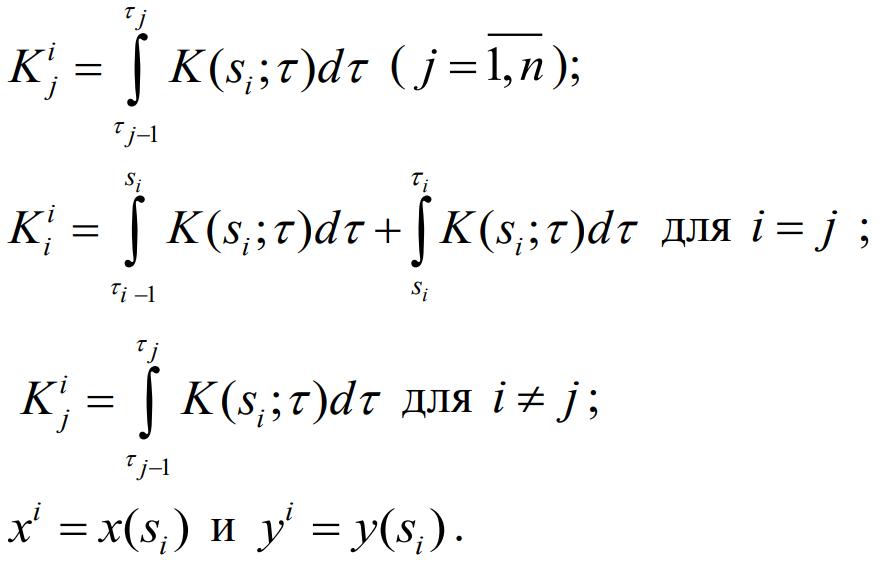
\includegraphics[width=0.5\linewidth]{../img/img1.png}}  \\
	\end{minipage}
\end{figure}

Используя эти обозначения и приближенное равенство \\${x_{*} \approx \sum_{j=1}^{n} x_{*}\left(s_{j}\right) \operatorname{spl}_{0}\left(A ;^{>} \mathbf{e}_{j}\right)=\sum_{j=1}^{n} x_{*}^{j} h_{j}}$, из уравнения (1) получаем его дискретный аналог, аппроксимирующий уравнение (1) при $h, \tau \rightarrow 0$, в виде СЛАУ 
\begin{equation}
\left\{\begin{array}{l}{x^{i}-\lambda \sum\limits_{j=1}^{20} K_{j}^{i} \cdot x^{j}=y^{i}} \\ {i=\overline{1,20}}\end{array}\right.
\end{equation}
Введём обозначения:
\begin{equation}
^>x=\left[x^{1}, \ldots, x^{20}\right\rangle,^>y=\left[y^{1}, \ldots, y^{20}\right\rangle \in ^>\mathbb{R}^{n}, F=\left(\delta_{j}^{i}-\lambda K_{j}^{i} \cdot h\right)_{20}^{20}=\left(f_{j}^{i}\right)_{20}^{20} \in L(\mathbb{R}, 20),
\end{equation}
где
\begin{equation*}
\delta_{j}^{i}=\left\{\begin{array}{l}{1, i=j} \\ {0, i \neq j}\end{array}\right.
\end{equation*}

Используя эти обозначения, СЛАУ перепишем в виде 

\begin{equation}
	F\cdot ^>x = ^>y
\end{equation}

Решая СЛАУ (4), получаем сеточную функцию $^>x=\left[x^{1}, \ldots, x^{20}\right\rangle \in ^>\underline{\mathbb{R}}^{|A|}(A)$, индуцирующую с помощью интерполяции приближенное решение уравнения (1). При $h \longrightarrow 0 (n \longrightarrow +\infty)$ такое приближенное решение в чебышёвской норме сходится к решению уравнения (1).

С помощью СЛАУ (4) находим численное решение интегрального уравнения.

\begin{align*}
^>x = [ 8.822711767, 5.060213014, 1.272657527,- 2.450440825,- 6.021091536,\\-
9.354906997,- 12.37309689,- 15.00433028,- 17.18642144,- 18.86779955,\\-
20.00872744,- 20.58224080,- 20.57478540,- 19.98653743,- 18.83139936,\\-
17.13667135,- 14.94240606,- 12.30046204,- 9.273278150,- 5.932397878]
\end{align*}

Приводим интегральное уравнение к краевой задаче для дифференциального уравнения 2-го порядка с постоянными коэффициентами. Имеем:

\begin{equation*}
	\left\{\begin{array}{l}x^{\prime \prime}(s)+\frac{2}{n-59} \frac{N+5}{N} x(s)=2 \frac{N+5}{N} \\ 
	x(0)=\frac{1}{n-59} \int\limits_{0}^{0} K(0, \tau) \cdot x(\tau) d \tau+y(0)=y(0) \\ 
	x\left(\frac{N+5}{N}\right)=\frac{1}{n-59} \int\limits_{0}^{\frac{N+5}{N}} K\left(\frac{N+5}{N}, \tau\right) \cdot x(\tau) d \tau+y\left(\frac{N+5}{N}\right)\end{array}\right.
\end{equation*}

\begin{equation*}
	\begin{cases}
		x^{\prime \prime}(s) + \frac{4}{3} x(s) = \frac{16}{3} \\
		x(0) = \frac{32}{3}\\
		x(\frac{8}{3}) = -4.134137784
	\end{cases}
\end{equation*}


Тогда аналитическое решение:

\begin{equation*}
	\begin{cases}
		x(s) = c_1 \sin(\sqrt{\frac{4}{3}} \cdot s) + c_2 \cos(\sqrt{\frac{4}{3}} \cdot s) + 4\\
		c_1 = -23.74378078\\
		c_2 = 6.666666667
	\end{cases}
\end{equation*}


Построим совмещённые графики:

\begin{figure}[H]
	\begin{minipage}[h]{1\linewidth}
		\center{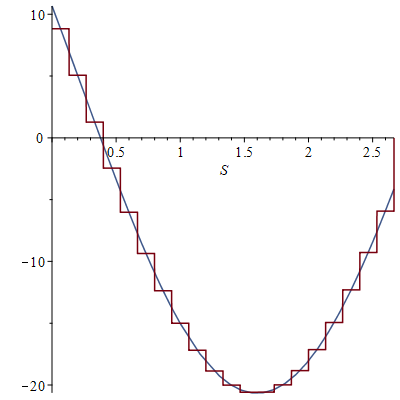
\includegraphics[width=0.75\linewidth]{../img/img2.png}}  \\
	\end{minipage}
\end{figure}


Максимальная абсолютная погрешность: $1.886427814$

Проверим:

\begin{figure}[H]
	\begin{minipage}[h]{1\linewidth}
		\center{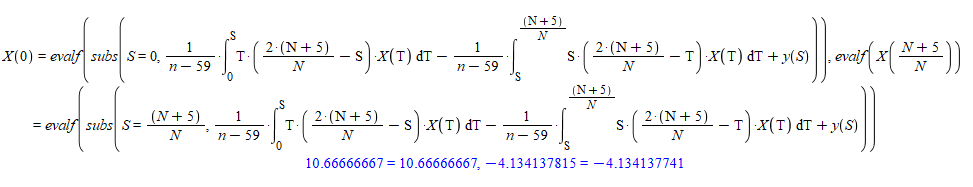
\includegraphics[width=1\linewidth]{../img/img3.png}}  \\
	\end{minipage}
\end{figure}

\textbf{Вывод.}\\
Применение метода коллокаций для приближенного решения интегрального уравнения Фредгольма 2-го рода с симметричным, непрерывным, аналитически заданным ядром допустимо и даёт хорошую точность численного решения.


\end{document}